\let\negmedspace\undefined
\let\negthickspace\undefined
\documentclass[journal]{IEEEtran}
\usepackage[a5paper, margin=10mm, onecolumn]{geometry}
%\usepackage{lmodern} % Ensure lmodern is loaded for pdflatex
\usepackage{tfrupee} % Include tfrupee package

\setlength{\headheight}{1cm} % Set the height of the header box
\setlength{\headsep}{0mm}     % Set the distance between the header box and the top of the text

\usepackage{gvv-book}
\usepackage{gvv}
\usepackage{cite}
\usepackage{amsmath,amssymb,amsfonts,amsthm}
\usepackage{algorithmic}
\usepackage{graphicx}
\usepackage{textcomp}
\usepackage{xcolor}
\usepackage{txfonts}
\usepackage{listings}
\usepackage{enumitem}
\usepackage{mathtools}
\usepackage{gensymb}
\usepackage{comment}
\usepackage[breaklinks=true]{hyperref}
\usepackage{tkz-euclide} 
\usepackage{listings}
% \usepackage{gvv}                                        
\def\inputGnumericTable{}                                 
\usepackage[latin1]{inputenc}                                
\usepackage{color}                                            
\usepackage{array}                                            
\usepackage{longtable}                                       
\usepackage{calc}                                             
\usepackage{multirow}                                         
\usepackage{hhline}                                           
\usepackage{ifthen}                                           
\usepackage{lscape}
\begin{document}

\bibliographystyle{IEEEtran}
\vspace{3cm}

\title{12.478}
\author{EE25BTECH11049 - Sai Krishna Bakki}
\maketitle
\vspace{-3em}
\textbf{Question:}\\
A force $\vec{P}=\myvec{2\\-5\\6}$ acts on a particle. The particle is moved from point $\vec{A}$ to point $\vec{B}$, where the position vectors of $\vec{A}$ and $\vec{B}$ are $\myvec{6\\1\\-3}$ and $\myvec{4\\-3\\-2}$ respectively. The work done is\\ 
\solution\\
Given
\begin{align}
    \text{Force } \vec{P}=\myvec{2\\-5\\6},\vec{A}=\myvec{6\\1\\-3},\vec{B}=\myvec{4\\-3\\-2}
\end{align}
Work done is given by
\begin{align}
    \vec{P}^T\brak{\vec{B}-\vec{A}}\\
    \implies \myvec{2&-5&6}\brak{\myvec{4\\-3\\-2}-\myvec{6\\1\\-3}}\\
    \implies \myvec{2&-5&6}\myvec{-2\\-4\\1}\\
    \implies -4+20+6=22
\end{align}
$\therefore$ The work done is 22 J.
\newpage
\begin{figure}
    \centering
    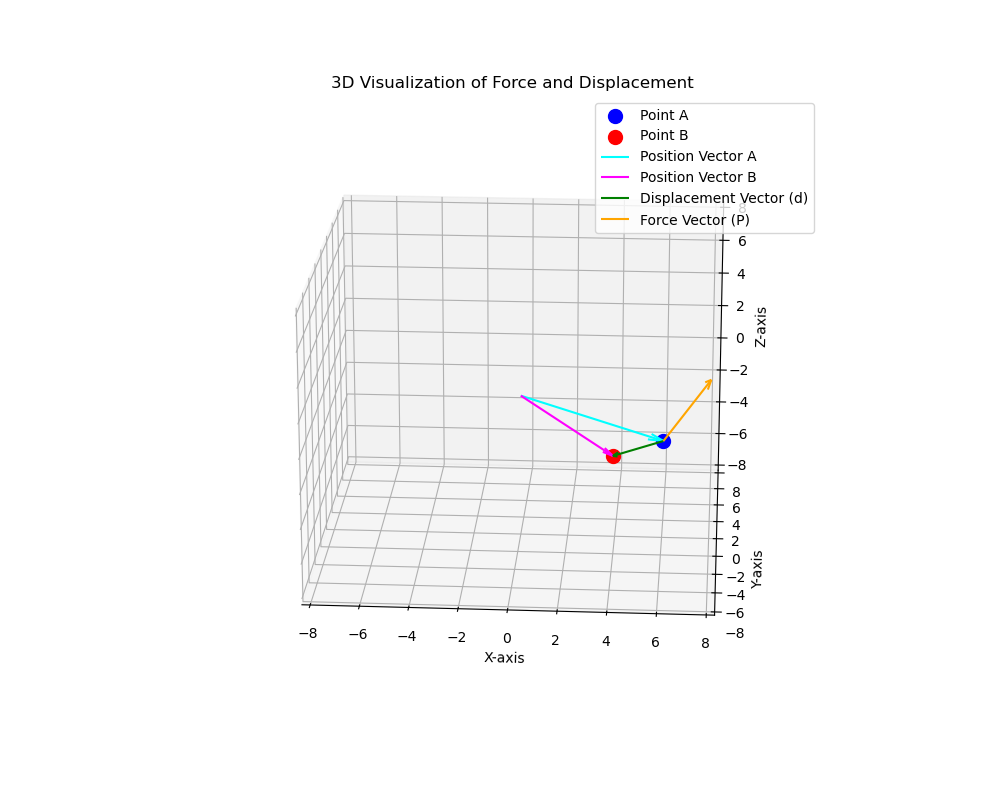
\includegraphics[width=1.1\columnwidth]{figs/Figure_1.png}
    \caption{}
    \label{fig:placeholder}
\end{figure}
\end{document}
